The figure \ref{2afiveeval} shows the prediction of $Y(\theta)$ conditional the 5 evaluation points, given in the project description, as a function of $\theta$. 

\begin{figure}
    \centering
    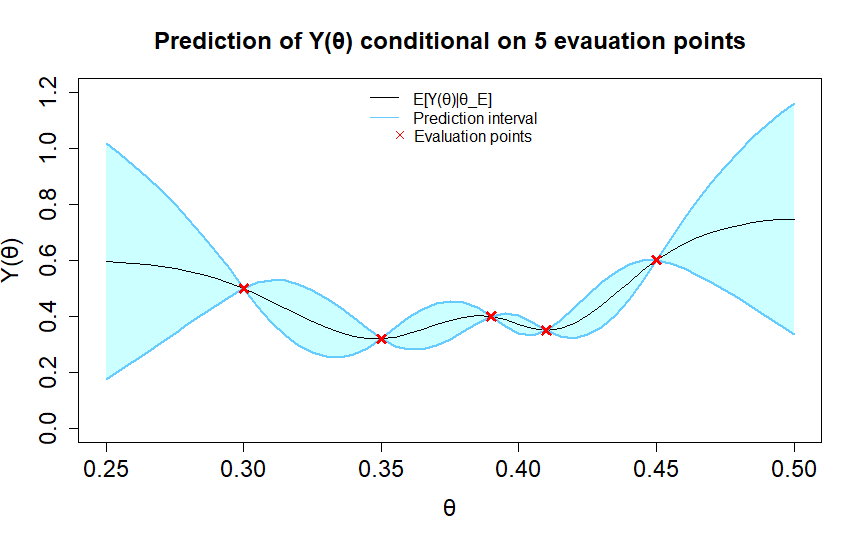
\includegraphics[width=100mm]{2aPlot.png}
    \caption{Prediction of $Y(\theta)$ conditional on the five evaluation points given. The graph includes a $90\%$ prediction interval. }
    \label{2afiveeval}
\end{figure}

%We can see that the evaluation points correspond well with the predicted $Y(\theta).$
